%! TEX program = pdflatex

\documentclass[oneside,solution]{tmpl}

\usepackage[utf8]{inputenc}
\usepackage[english,ukrainian]{babel}

\title{Домашня робота}
\author{Захаров Дмитро}
\studentID{МП-31}
\instructor{Ігнатович С.Ю.}
\date{\today}
\duedate{23:59 10 березня, 2024}
\assignno{4}
\semester{Весняний семестр 2024}
\mainproblem{Диференціальні рівняння як моделі процесів}

\begin{document}

\maketitle

% \startsolution[print]

\problem{Використання популяційної моделі.}

\textbf{Умова.} Кількість населення Землі зараз складає приблизно $N_0=8 \; \text{млрд}$ людей, а щоденний ($\Delta t = 1 \; \text{день}$) приріст дорівнює приблизно $\Delta N = 200 \; \text{тисяч}$ людей. Припустимо, що швидкість, з якою збільшується населення, пропорційна кількості людей, і коефіцієнт пропорційності не змінюється. 

\begin{enumerate}
    \item Якою буде кількість людей у $2050$ році?
    \item Коли кількість людей досягне $N = 50 \; \text{млрд}$?
    \item З'ясуйте, чи сильно зміниться результат підрахунків, якщо врахувати або не врахувати високосні роки.
    \item З'ясуйте, наскільки відрізняються результати, отримані з міркувань диференціального рівняння і з міркувань різнецевого рівняння.
\end{enumerate}

\textbf{Розв'язок.} 

\textit{Пункт 1.} Нехай $n(t)$ -- залежність кількості населення у млрд від часу $t$ у роках, що відкладений від $2024$ року. За умовою, рівняння динаміки зміни кількості населення:
\begin{equation}
    \dot{n} = \kappa n \implies n(t) = n(0)\exp(\kappa t)
\end{equation}

За умовою $n(0)=N_0$, тому $n(t)=N_0\exp(\kappa t)$. Залишилось знайти $\kappa$, що ми зробимо через умову на щоденний приріст. Помітимо, що величина $\dot{n}(t)$ показує миттєвий приріст населення у момент часу $t$. За умовою ми знаємо, що зараз (тобто у момент часу $t=0$) приріст дорівнює $\Delta N/\Delta t$, тому:
\begin{equation}
    \dot{n}(0) = \frac{\Delta N}{\Delta t} \implies \kappa N_0 = \frac{\Delta N}{\Delta t} \implies \kappa = \frac{\Delta N}{N_0 \Delta t}
\end{equation}

Тому остаточно рівняння кількості населення від часу:
\begin{equation}
    n(t) = N_0 \exp\left( \frac{\Delta N \cdot t}{N_0 \cdot \Delta t}\right)
\end{equation}

Підставимо числа кількісно. Маємо $N_0=8$, $\Delta N = \frac{2 \cdot 10^5}{10^9} = 2 \cdot 10^{-4}$ і нарешті час $\Delta t = \frac{1}{365}$, тому
\begin{equation}
    n(t) \approx 8 \exp (0.009125\cdot t)
\end{equation}

$2050$ рік відповідає моменту часу $t=26$, тому шукана відповідь:
\begin{equation}
    n(26) \approx 8 \exp(0.009125 \cdot 26) \approx \boxed{10.14 \; \text{млрд}}
\end{equation}

\textit{Пункт 2.} У цьому пункті потрібно розв'язати рівняння $n(\tau)=N$ відносно $\tau$. Оскільки залежність $n(t)$ явно задана, то зробити це просто:
\begin{equation}
    N_0 \exp \left(\frac{\Delta N \cdot \tau}{N_0 \cdot \Delta t}\right) = N \implies \tau = \frac{N_0 \cdot \Delta t}{\Delta N} \log \frac{N}{N_0},
\end{equation}
де через $\log$ позначено логарифм за основою $e$. Залишається підставити числа:
\begin{equation}
    \tau = \frac{8}{365 \cdot 2 \cdot 10^{-4}}\log \frac{50}{8} \approx 200
\end{equation}
Отже, така кількість населення буде приблизно у $\boxed{2224}$ році.

\textit{Пункт 3.} Навіть не проводячі конкретні підрахунки, питання важливості враховування або не враховування високосних років не дуже змістовне. Якщо навіть припустити, що це викликає похибку, є дуже багато факторів окрім цього, що впливають на порядок більше:
\begin{itemize}
    \item Чи дійсно населення складає саме $8 \; \text{млрд}$ і на скільки можна довіряти демографічним данним? В деяких країнах порахувати кількість взагалі дуже складно, тому точність наврядше можна сказати більше ніж в десятках тисячах. В багатьох випадках, ці числа взагалі лише є оцінками (як, наприклад, взяті нами $8 \; \text{млрд}$).
    \item Коли ми беремо, що приріст є приблизно 200 тисяч людей на день -- це інша оцінка, що скоріше за все була попередньо усереднена по іншим джерелам. Звичайно, що щоденний приріст кожного дня є різним і оцінити таку величину теж не можна абсолютно точно.
    \item Напевно, головна проблема -- це обрана модель. Чи дійсно ми маємо чисту експоненту? Хоч це і достатньо непогане наближення, проте насправді модель росту популяції значно складніша і наш обраний коефіцієнт $\kappa$ не є постійним.
\end{itemize}

Проте, нехай ми розглядаємо нашу ідеалізовану задачу і вирішили врахувати високосний рік. Основне місце, де ми його враховували -- це коли знаходили значення $\Delta t$ у роках. Нехай ми вирішили взяти $\Delta \widetilde{t} = \frac{1}{365.25}$ і підставити у залежність $n(t)$:
\begin{equation}
    \widetilde{n}(t) \approx N_0 \exp\left(\frac{\Delta N \cdot t}{N_0 \cdot \Delta\widetilde{t}}\right) \approx 8 \exp (0.00913125 t)
\end{equation}
Знайдемо відносну різницю:
\begin{equation}
    \epsilon = \frac{\widetilde{n} - n}{n} = \frac{\widetilde{n}}{n}-1 = \exp(6.25 \cdot 10^{-6} \cdot t) - 1
\end{equation}
Отже, якщо взяти навіть $t=100$, то відносна різниця $\epsilon \approx 0.063 \%$ -- нехтовна величина. 

\textit{Пункт 4.} Розглянемо різнецеве рівняння, де $n[d]$ позначає населення у день $d$ (щоб відрізняти неперервну залежність $n(\cdot)$ від дискретної $n[\cdot]$, ми пишемо різні дужки). Тоді, динаміка зміни кількості населення:
\begin{equation}
    n[d+1] = (1+\beta)\cdot n[d],
\end{equation}
де $1+\beta$ -- коефіцієнт росту населення. За умовою, $n[1] = n[0] + \Delta N$ та $n[0]=N_0$, звідки отримуємо:
\begin{equation}
    n[1] = (1 + \beta)N_0 = N_0 + \Delta N \implies \beta = \frac{\Delta N}{N_0}
\end{equation}
Також, добре видно, що
\begin{equation}
    n[d] = (1+\beta)^d \cdot n[0]
\end{equation}

Тому остаточно:
\begin{equation}
    n[d] = N_0\left(1+\frac{\Delta N}{N_0}\right)^d 
\end{equation}

Тепер спробуємо порахувати перший пункт з урахуванням такої залежності. 2050 рік буде через $26$ років, а отже приблизно $26\cdot 365 = 9490$ днів, тому
\begin{equation}
    n[9490] = 8 \cdot \left(1+\frac{2 \cdot 10^{-4}}{8}\right)^{9490} \approx 10.14 \; \text{млрд},
\end{equation}
що майже не відрізняється від попередньо отриманого результату. 

Чому так трапилось? Позначимо $\frac{\Delta N}{N_0 \Delta t}$ через $\zeta \approx 0.009 \ll 1$. Тоді, неперервна величина має вигляд:
\begin{equation}
    n(t) = N_0 \exp (\zeta t) = N_0 \sum_{k=0}^{\infty} \frac{\zeta^k t^k}{k!}
\end{equation}
Тепер подивимось на $n[d]$. Якщо нам потрібно отримати кількість через $t$ років, то нам треба знаходити $n[d_t]$, де $d_t=t/\Delta t$ (якщо вважаємо $\Delta t = 1/365$, то $d_t \in \mathbb{N}$) тобто 
\begin{equation}
    n[d_t] = N_0\left(1 + \zeta\Delta t\right)^{t/\Delta t} = N_0 \sum_{k=0}^{d_t} C_{d_t}^k (\zeta \Delta t)^k
\end{equation}

Далі помітимо, що $\zeta^2$ -- нехтовна величина, тому ми можемо записати:
\begin{equation}
    n(t) \approx N_0(1 + \zeta t), \; n[d_t] \approx N_0(1 + d_t\zeta \Delta t)=N_0(1+\zeta t)
\end{equation}
Отже, дійсно отримали, що $n(t) \approx n[d_t]$, якщо вважати $\zeta^2$ малою величиною (що дійсно є так). Якщо нехтувати $\zeta^3$, то відмінність вже буде:
\begin{gather}
    \frac{n(t)}{N_0} \approx 1 + \zeta t + \frac{\zeta^2 t^2}{2} \\
    \frac{n[d_t]}{N_0} \approx 1 + \zeta t + \frac{d_t(d_t-1)\zeta^2\Delta t^2}{2}
\end{gather}

Отже,
\begin{equation}
    \frac{n(t)}{N_0} - \frac{n[d_t]}{N_0} \approx \frac{\zeta^2t\Delta t}{2} \approx 1.1 \cdot 10^{-7}\cdot t,
\end{equation}
що є дуже малим відхиленням.

\problem{Альтернативна популяційна модель.}

\textbf{Умова.} Диференціальне рівняння $\dot{x}=a\left(1-\frac{x}{K}\right)$ теж може використовуватися у популяційній динаміці. Нарисуйте ескіз графіків розв'язків цього рівняння, не розв'язуючи його. В чому відмінність цих розв'язків від розв'язків логістичного рівняння $\dot{x}=ax\left(1-\frac{x}{K}\right)$?

\textbf{Розв'язок.} Нехай ми задаємо значення $x_0=x(0)$ -- початкову популяцію. Одразу видно, що якщо $x_0=K$, то $\dot{x}(0)=0$ і тому графік буде просто горизональною прямою $x(t) \equiv K$. В цьому схожість заданого сімейства розв'язків з сімейством розв'язків $\dot{x}=ax\left(1-\frac{x}{K}\right)$, де ситуація при $x(0)=K$ аналогічна. 

Отже, нехай $x_0<K$. Тоді $\dot{x}(0) > 0$, тому кількість популяції почне зростати, причому буде зростати асимптотично до прямої $x \equiv K$. Дійсно, для усіх $x \in [0,K)$ похідна додатня, тому функція $x(t)$ монотонно зростає, але $\lim_{x \to K^-}\dot{x} = 0$, тому крива вийде на пряму (окрім того, $x(t)$ не буде перетинати цю пряму, міркуючи аналогічно, як це було зроблено на лекції). 

Для $x_0>K$ ситуація симетрична -- $x(t)$ буде зменьшуватись асимптотично до $x \equiv K$. 

Ескізи графіків для $K=1$ зображені на рис. \ref{fig:sol}.

\begin{figure}
    \centering
    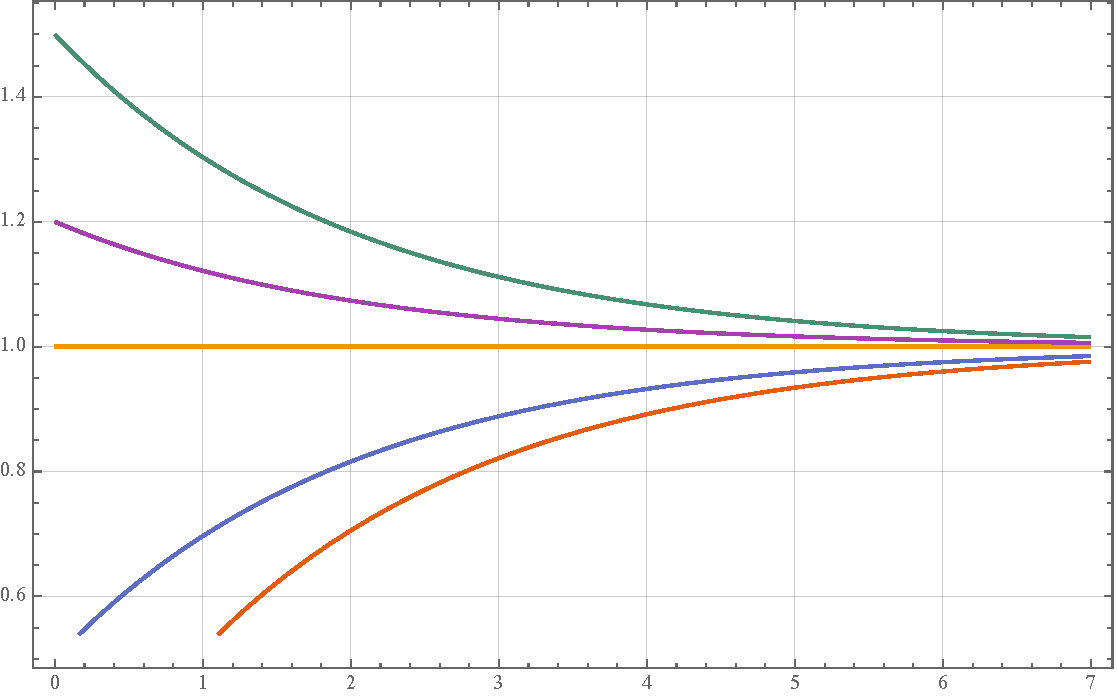
\includegraphics[width=0.7\textwidth]{images/hw_3/sol.pdf}
    \caption{Ескіз розв'язків рівняння $\dot{x}=a(1-\frac{x}{K})$ при $K=1$. Жовта лінія відповідає початковій умові $x_0=K=1$, синя та червона -- $x_0<K$, зелена та фіолетова -- $x_0>K$.}
    \label{fig:sol}
\end{figure}

Також, для самоперевірки, можемо отримати конкретні розв'язки:
\begin{equation}
    x(t) = K + (x_0-K)\exp\left(-\frac{at}{K}\right)
\end{equation}
Як бачимо, дійсно $\lim_{t \to \infty}x(t) = K$, причому знак $\dot{x}=a(1-\frac{x_0}{K})e^{-at/K}$ визначається виключно знаком виразу $1-\frac{x_0}{K}$.

Головна відмінність від розв'язків $\dot{x}=ax(1-\frac{x}{K})$ -- відсутність точки перегину. Дійсно, навіть користуючись початковим рівнянням без розв'язків:
\begin{equation}
    \ddot{x} = \frac{d}{dt}\dot{x} = \frac{d}{dt}\left(a\left(1-\frac{x}{K}\right)\right) = -\frac{1}{K}\cdot \dot{x}.
\end{equation}
Оскільки $\dot{x} = 0$ лише коли $x_0=K$, то $\ddot{x} \neq 0$ і тому точки перегину немає. В свою чергу, $\dot{x}=ax(1-\frac{x}{K})$ може мати точки перегину, як добре видно по ескізам з лекції.

\end{document}
